\documentclass[bsc,frontabs,twoside,singlespacing,parskip]{infthesis} 
\usepackage{graphicx}
%\usepackage{natbib}
\graphicspath{ {images/} }


\begin{document}

\title{Text Driven Talking Heads}

\author{Iain Brown}
\course{Computer Science}
\project{Undergraduate Dissertation} 
%\project{Undergraduate Thesis} % AI%Psy
%\project{4th Year Project Report}

\date{\today}
%\abstract{The aim of this project is to build a head motion synthesizer for a lifelike animated avatar. The head motions will be predicted entirely from the text of transcribed speech with the aim of finding a mapping between the text and natural head motions. Unlike previous areas of research where the head motions are generated from recorded speech.}
\maketitle
%\section*{Acknowledgements}
%Acknowledgements go here. 
\tableofcontents

% ============================================================= %
\chapter{Introduction}

The Introduction chapter should always provide a 'roadmap' to the report. Of course it should provide an introduction to the problem being considered, but it should also give some details of what you did - do not leave this to the conclusion. You should give forward references into the rest of the report - e.g., "In Chapter 2 how algorithms and heuristics are used to deal with approximate counting are discussed", "The design of the system is presented in Chapter 4", "In Chapter 3 the reasons for choosing to focus on the bounded-degree case of this problem are explained"


- Head motion is very important when it comes to human communication \\
- Dialogue is much harder to fully understand without the non-verbal information \\
- Generating Lifelike avatars in many applications, VR, video games, shopping assistant \\
- Realistic head motions are vital otherwise humans may feel weird interacting with an avatar \\
- Project aimed to create a system that synthesises natural head motions just from the text \\
- Without knowledge present in speech \\
- Using Various Natural Language Processing Techniques \\

% ============================================================= %
\chapter{Background Information}

\section{Human Computer Interaction}

Human Computer Interaction is a field of Computer Science in constant change. With the goal of enhancing Human Computer Interaction researchers have looked to the field of Embodied Conversational Agents, where an intelligent agent is mapped to a graphical animation or body to replicate the most natural of interactions: face to face dialogue. \cite{ecas} 

Embodied Conversational Agents have had been found to enhance the interactions with computers \cite{conv_agents} and researchers are perpetually improving systems in order to increase user satisfaction. One of the biggest benefits to using an ECA is that the interaction is of a social nature, being more familiar to humans and aids the systems perceived trust worthiness, allowing a richer interaction between the user and the computer. Also the intelligibility of speech produced in noise is also improved when a speaker's face is visible \cite{emotion_head_motion}, this means that because the user has a physical representation of the ECA they can more easily understand what the agent is saying rather than if it was just speech output. These results suggest that nonverbal gestures such as head movements play a more direct role in the perception of speech than previously known. \cite{vis_prosody}

There are some limitations to consider when talking about ECA's, mainly to do with what Masahiro Mori called the Uncanny Valley effect. Mori states that the familiarity with a robot or graphic representation of an avatar increases in correlation with the rise of human likeliness, but there is a distinct fall in familiarity before achieving a life-like human representation referred to as the Uncanny Valley which causes revulsion in humans. \cite{uncanny}

\begin{figure}[h!]
	\centering
	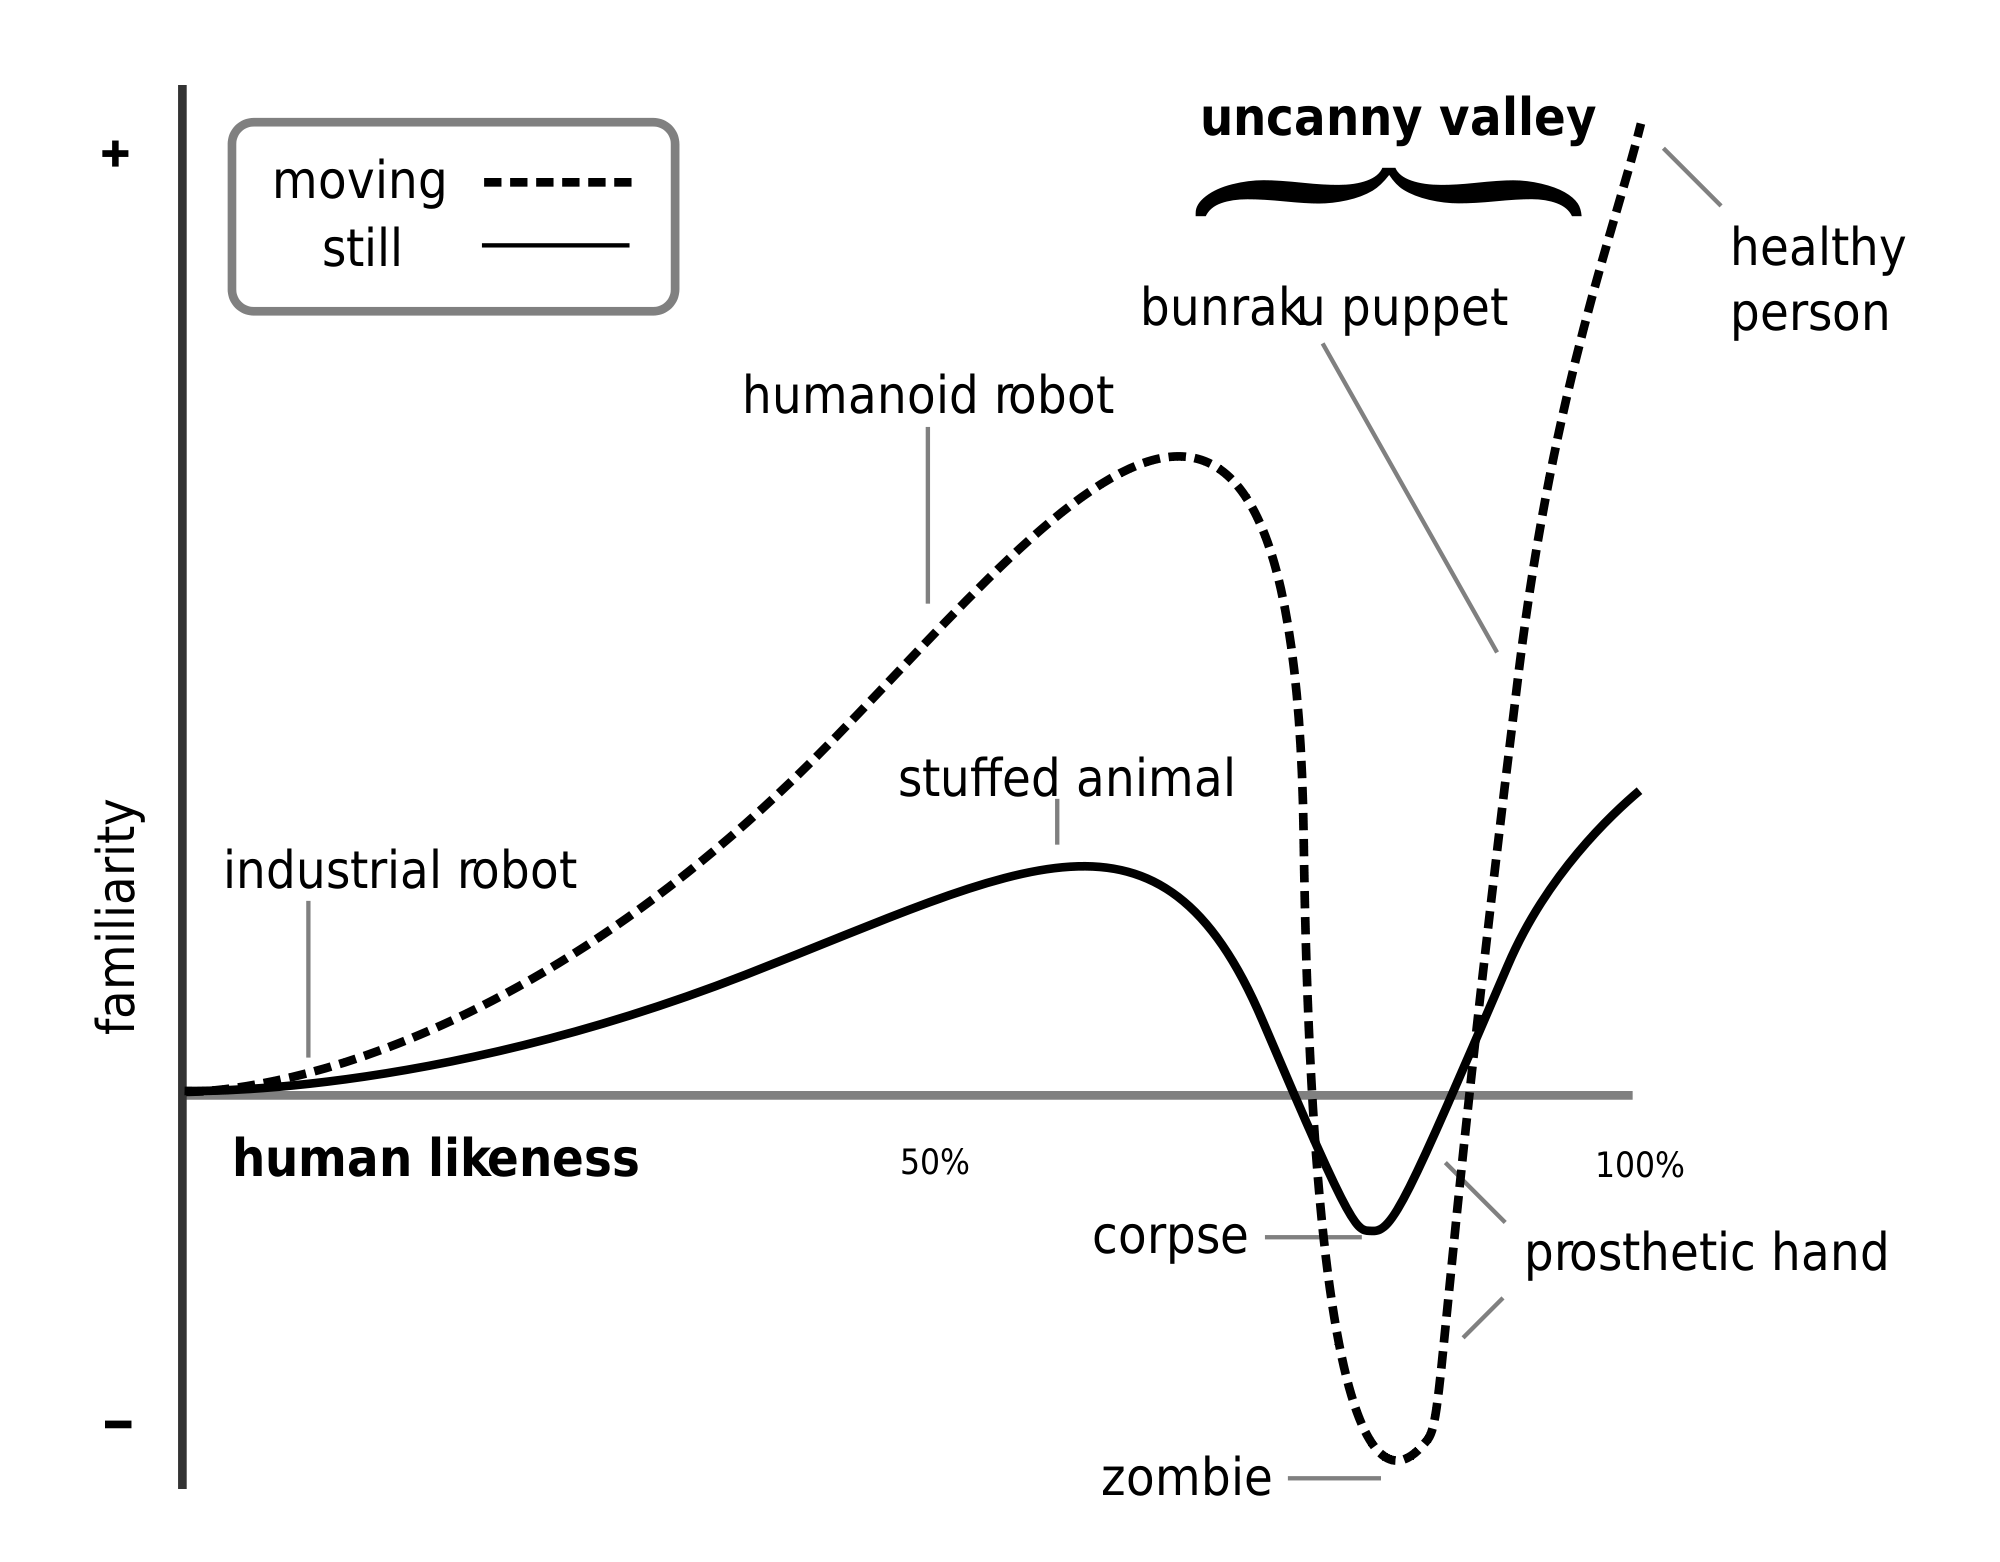
\includegraphics[width=0.6\textwidth]{uncanny}
	\caption{The Uncanny Valley effect}
\end{figure}

\section{Data and Task}

The task for the project was as follows: Using only text transcriptions of speech can we synthesise life-like head motions that seem realistic and natural to humans. The project aimed to investigate the correlation between head motions and the information present in speech unique to the speaker. The difficulty of the task comes from the lack of unique information about the speech, as we are only using the transcribed text. To tackle this we will be using a Text-to-Speech system called Festival that analyses the text and 

\subsection{Data Recordings}

The data used for the project was data recordings from the Centre of Speech and Technology Research at Edinburgh University. The recordings consisted of optical motion capture sessions in which participants wore 4 reflective markers on their torso and a hat with 3 reflective markers. There were 7 V100:R2 cameras that tracked the reflective markers at a sampling rate of 100Hz. Participants were asked to read out transcriptions of fairy tales.

\begin{figure}[h!]
	\centering
	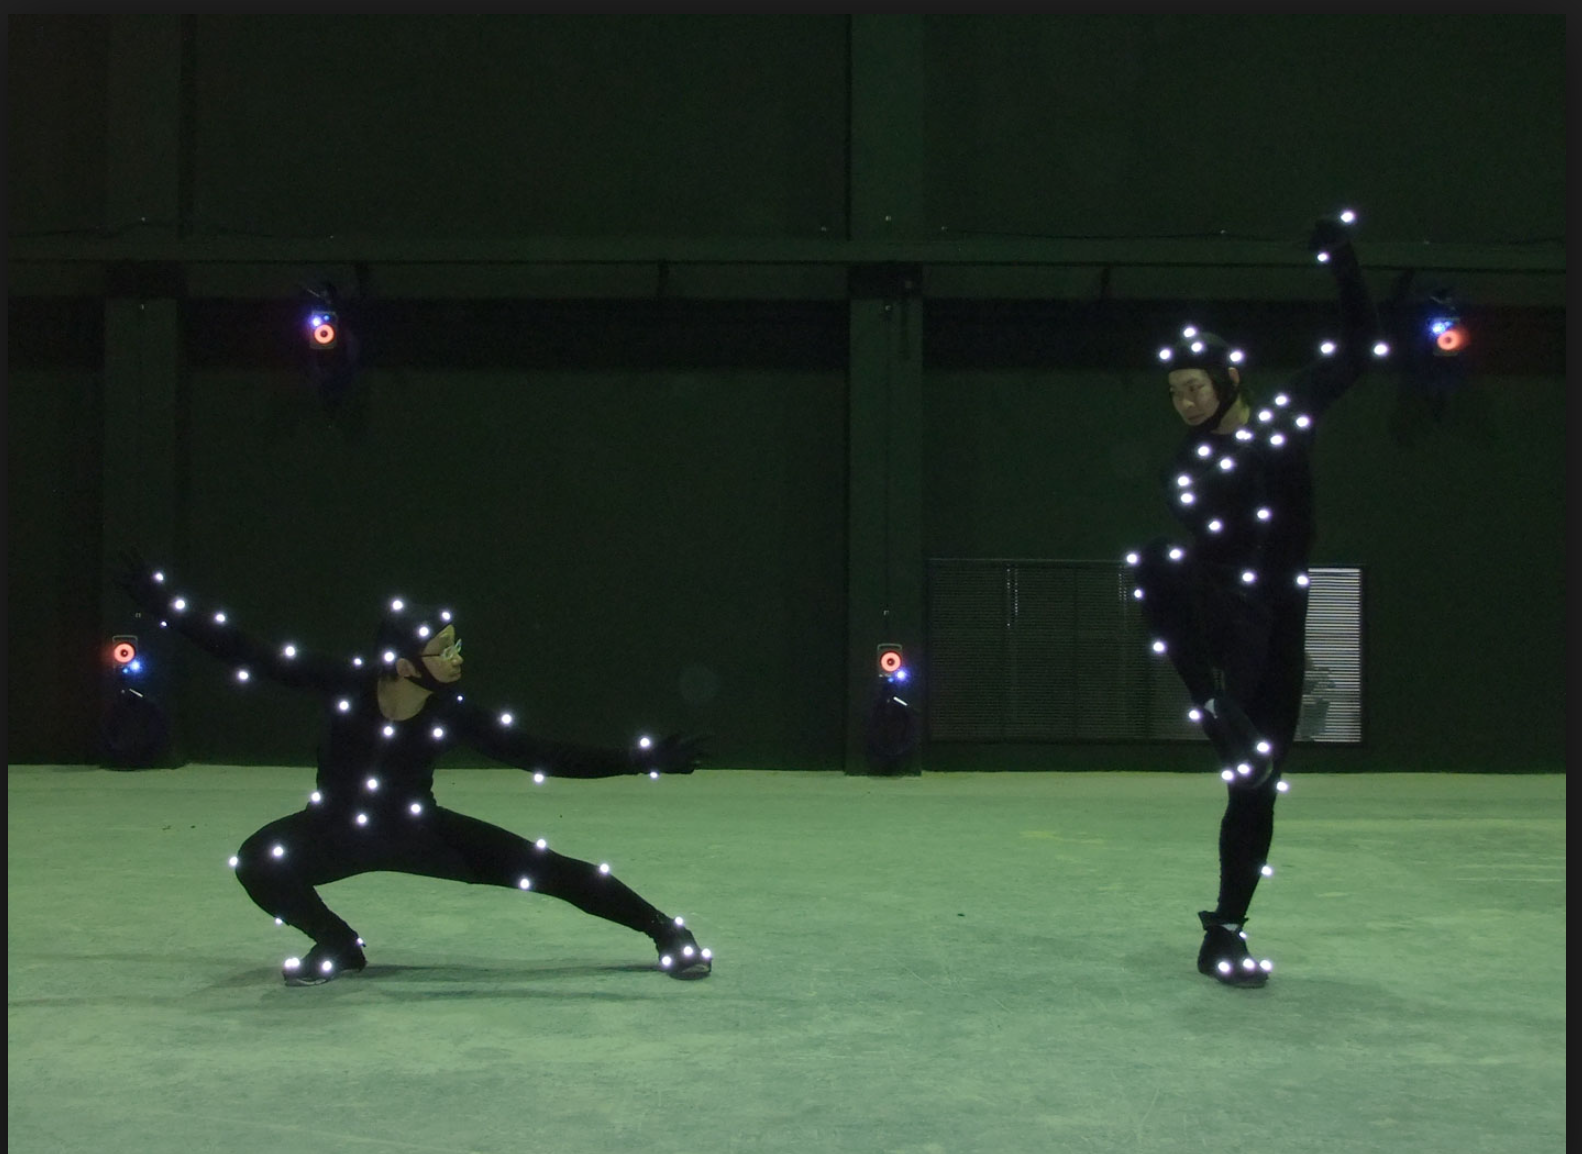
\includegraphics[width=.5\textwidth]{mocap.png}
	\caption{Setup of the mo-cap environment}
\end{figure}

\section{Festival}

Festival applies various Natural Language Processing techniques to the text to generate information  so that it can synthesise speech.  There are many steps in this pipeline, each adding a little bit more information to the text before Festival can then apply signal processing to generate audio. 

- Natural Language Processing Techniques \\
- Tokenisation \\
- Pos tags \\
- Phrase Break Prediction \\
- Phonetics \& Phonology \\
- Generating pronunciations \\
- Letter to sound rules\\
- Syllabification\\
- Duration based on classification and regression trees \\
Festival generates pronunciations by performing syllabification, breaking the sentences and words into syllables and looking up phonemes in a lexicon to determine their pronunciations. Using this information the system can generate ToBi markers, 

\begin{figure}[h!]
	\centering
	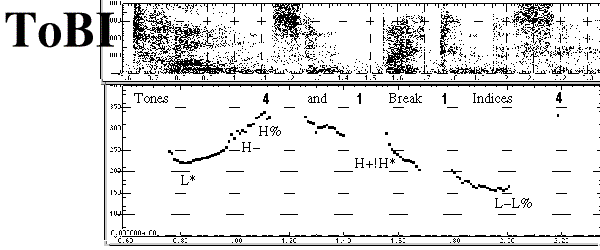
\includegraphics[width=1\textwidth]{tobi.png}
	\caption{ToBi Markers}
\end{figure}

\section{Euler angles}

Euler angles are three angles that represent the orientation of a rigid body in 3-Dimensional space, typically referred to as 'yaw', 'pitch' and 'roll'. Euler angles allows us to reduce the number of parameters normally used to represent rigid body orientation down to 3 parameters. It is a very popular method because of the reduced complexity and is commonly used in robotics and 3D animation software because of this. As the project focused on rigid head motions there was no translation taken into account when designing the 3D avatar head motions. This allowed the project to use Euler angles as the sole units of movement in the project.

\begin{figure}[h!]
	\centering
	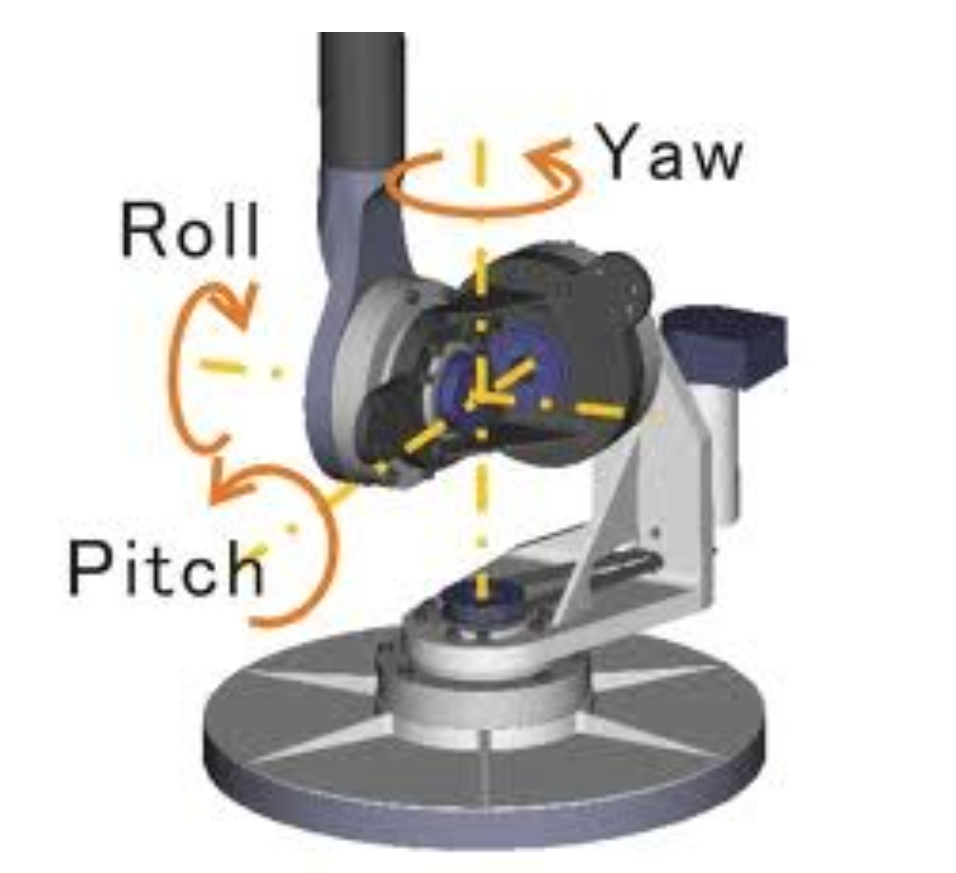
\includegraphics[width=.5\textwidth]{euler_angles.png}
	\caption{Euler Angles in Robotics}
\end{figure}


\section{Poser Animation}

3D animation and rendering software was used to visualise the generated head motions. The software used for this purpose was PoserPro 2012 by Smith Micro Software, a 3D animation tool with the emphasis on character creation and animation. PoserPro allows users to animate body parts of 3D characters and change their characteristic like rotation, translation and scale, meaning that the head of a character could be moved independently with ease.

With a scripting plug-in for Python called PoserPython, \cite{poser_python} allowing users to create scripts to manipulate objects and characters in the scene using Python was one of the main reasons for choosing PoserPro over other animation and rendering software like Blender. Poser also uses Euler angles as it's unit of rotation.


\begin{figure}
	\centering
		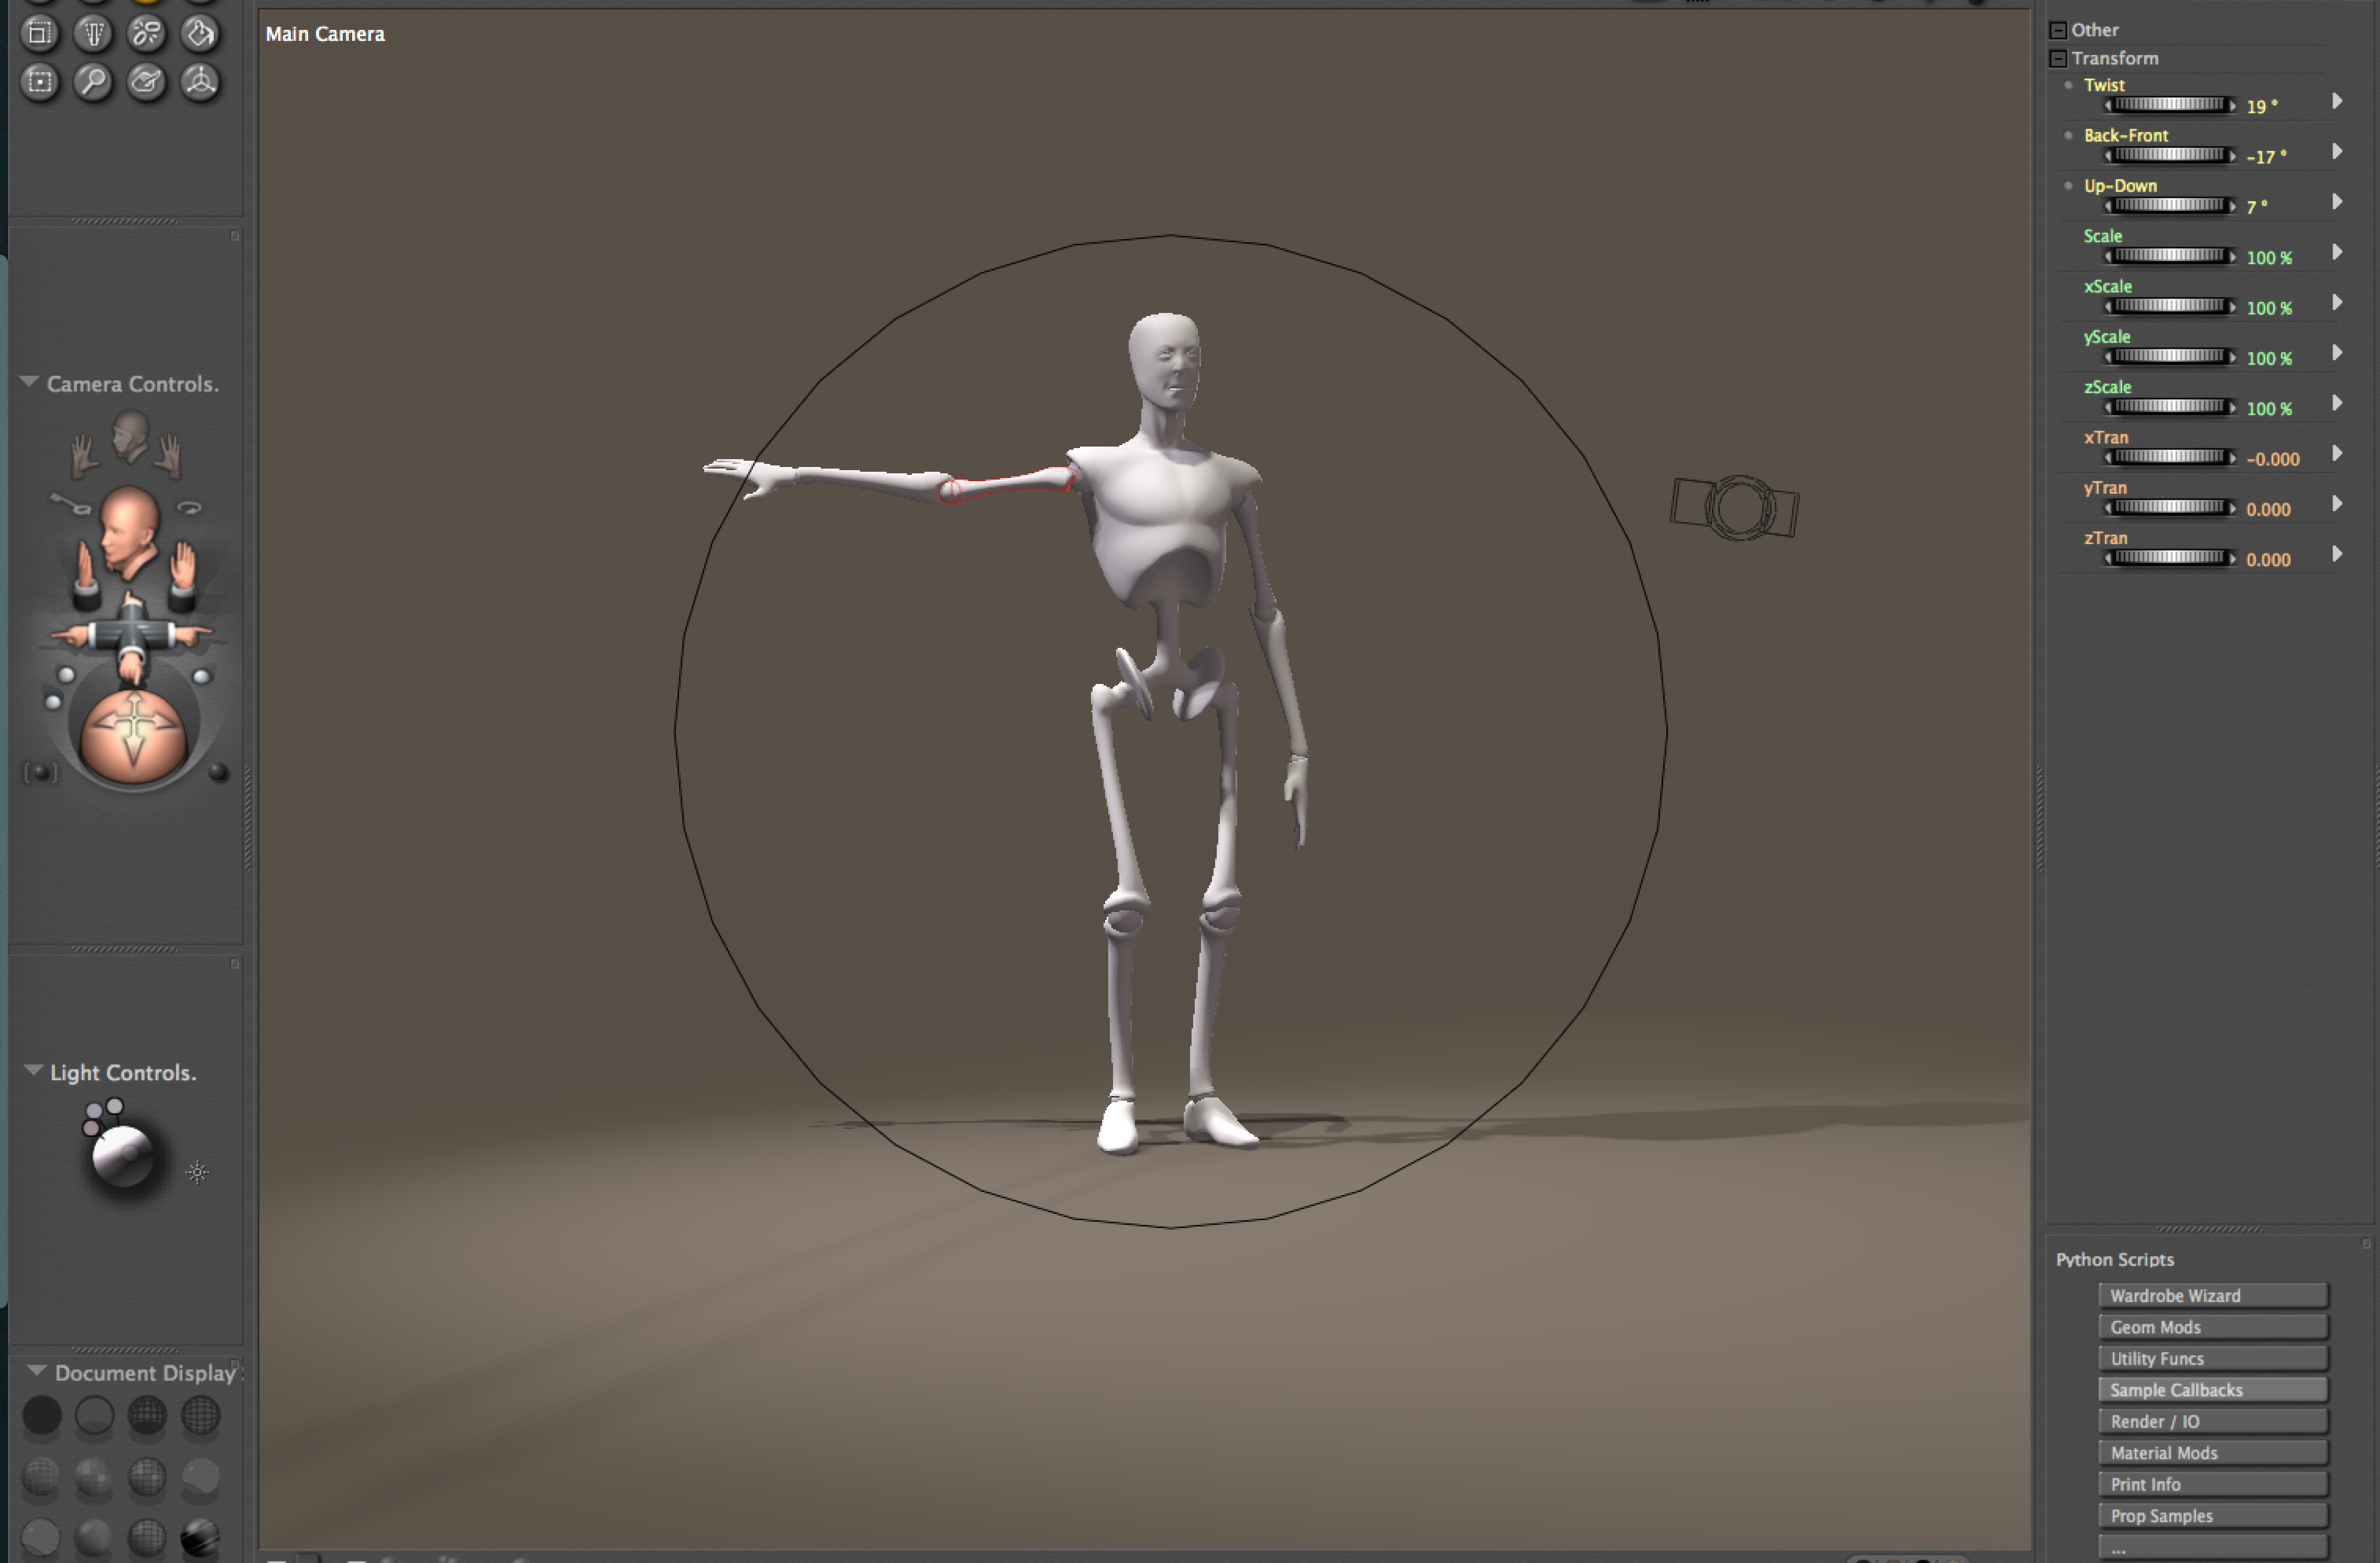
\includegraphics[width=1.0\textwidth]{poser.png}
		\caption{Overview of Poser Pro}
\end{figure}

% ============================================================= %
\chapter{Text-Driven Head Motion Synthesis}
% This will be the theoretical implementation details 

% - To develop a system that is capable of synthesising a life-like talking head from text.
% - use a text to speech system to symnthesize the audio and save data about the audio
% - Build a mapping of words and sentences to discrete head motions
% - Make the system similar to real life (i.e recorded speech)
% - use Poser to animate the head motions
%The goal of this project was to develop a system that was capable of synthesising life-like, realistic head motions from transcribed speech. The project aimed to 

\section{Hypotheses}

To build a system that was capable of synthesising real-life head motions from text, hypotheses about the relation of head motion events and speech content were introduced. The system built on these hypotheses, linking them together in order to synthesis the final head motions. 

\cite{first_paper} 
- Primary head motion to be nodding \\

\subsection{Prosodic Features}

--about prosody-- 

Head motions correlate strongly with prosody present in speech \cite{vis_prosody}. My first hypothesis relates to the rate of change of the fundamental frequency present in the synthesised speech. This is indicated in the Festival output as values around 120 Hz for male voices and 210Hz for female voices \cite{f0_values}. Sudden changes in the frequency should be reflected in head motions. For example in the intonation falls the head should lower accordingly \cite{Kendon}.

\subsection{Phrasing}

--about phrasing--

Phrasing plays a huge role in how something is said. It has been found that nodding head motions frequently occur at the end of phrases or at strong phrase boundaries, especially if the speaker is confident in what they are saying. \cite{ishi2008}  

\subsection{Sentiment Analysis}

Sentiment analysis is a popular area of natural language processing. It is often used to gauge reviews for products\cite{sentiment_online} and films\cite{sentiment_films} due to the availability of data and ease of tagging the reviews as either positive or negative.

Sentiment or emotion in speech has various effects on head motions. In a study It was found that the absence of head motion can be easily identified as 'neutral' emotion. \cite{emotion_head_motion} whereas participants in the study found it difficult to differentiate between head motions that were typical of 'happy' and 'sad' emotions. This study shows that emotive analysis on the text should be treated as an 'intensifier' of the underlying head motions derived form other areas of the text rather than altering the head motions to fit an emotion.



\subsection{Text Content}

There are two types of gestures that relate to speech. \cite{lexical_gestures} The first are motor movements which are typically simple, brief, repetitive and have a high correlation with prosodic features. The other type are lexical movements, gestures that help the speaker mentally perform lexical lookups subconsciously. These gestures are very different to motor movements and are much longer, more complex and relate more to the lexical information in the speech. To portray these ideas in this project 

\cite{kendon} Gesture as Utterance\\

\section{Text analysis}
\subsection{Festival}

\section{Head Motion Synthesis}

% ============================================================= %
\chapter{Implementation}

- Had to tie in a lot of things together \\
- Implemented the project using python \\
- Sub process calls \\
- LISP scripts for Festival \\
- Had to alter LISP Scripts to save audio files \\
- Pre-existing scripts for data preparation \\
- Downsampling

\begin{figure}
	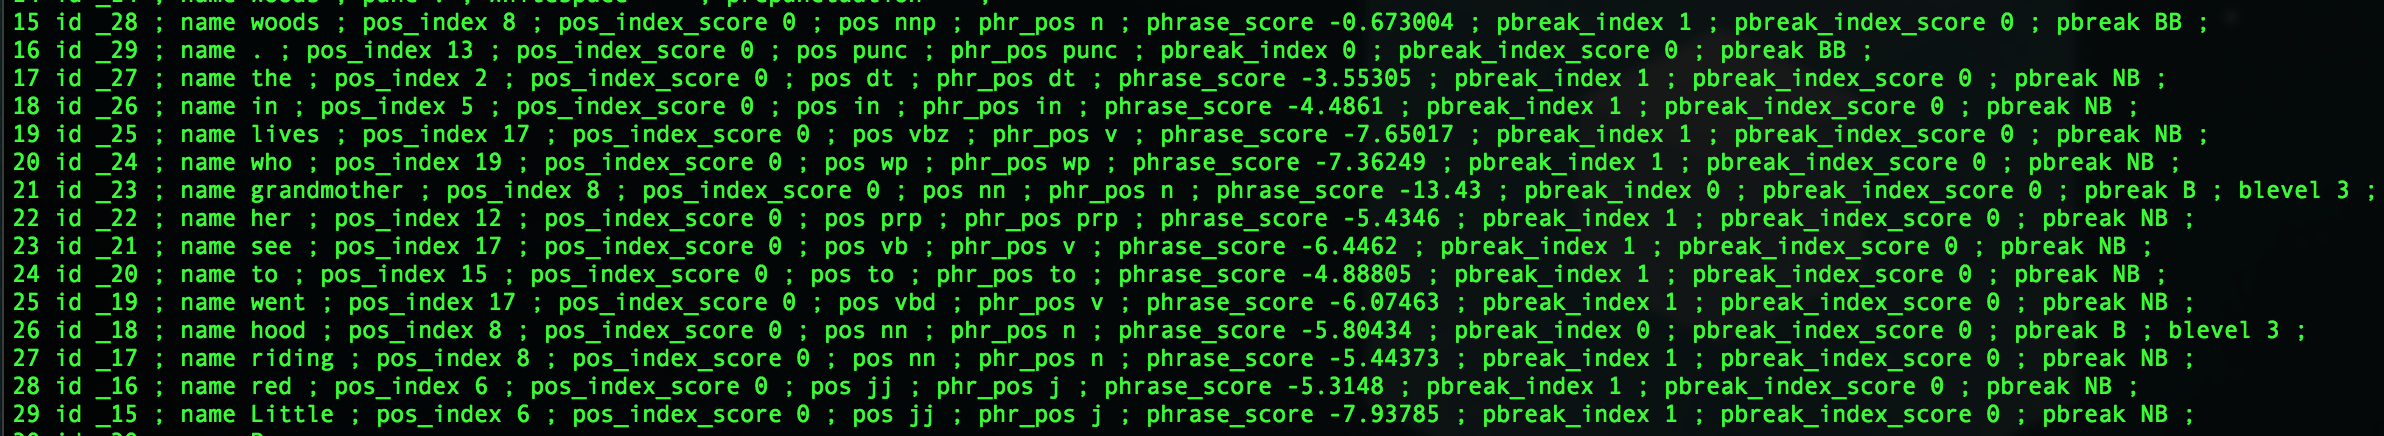
\includegraphics[width=1.1\textwidth]{festival_output.png}
	\caption{Output from festival analysis}
\end{figure}



\section{Basic System}
-The most basic head motion is nodding \\
- Paper - first one about head motions \\
- We want the avatar to seem familiar \\
- So we want to apply nodding \\

\subsection{Trignomietric Functions}
- Nodding motion similar to sine wave \\
- So for the basic system used sine wave formula to change just one Euler angle \\

\section{Random System}

\subsection{Discrete Head Motions}
- Represent Head Motions as discrete N dimensional vectors \\
- Apply smoothing methods to generate overall head shape \\
- Looked into Spherical Linear interpolation \\
\cite{rigid_head_motion}
- Correlation with words


\subsection{Bezier Smoothing}

- Went with Bezier smoothing, similar to SLERP\\
- INTERPOLATION
- Bezier Formula
- Bezier doesn't reach the discrete points\\
- This was good for the head motions \\

\begin{figure}
	$$ B(t) = \sum_{i=0}^n {n \choose i} (1-t) t^i P^i $$
	\caption{Recursive Bezier Definition} 
\end{figure}

\begin{figure}
	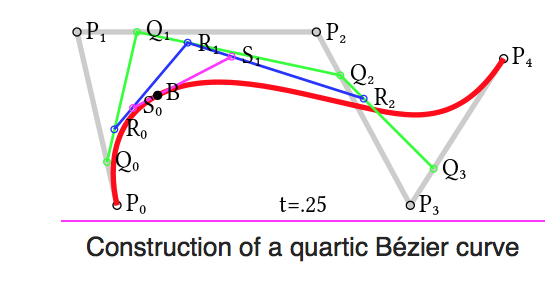
\includegraphics[width=1\textwidth]{bezier_example.png}
	\caption{Example of Bezier}
\end{figure}

\begin{figure}
	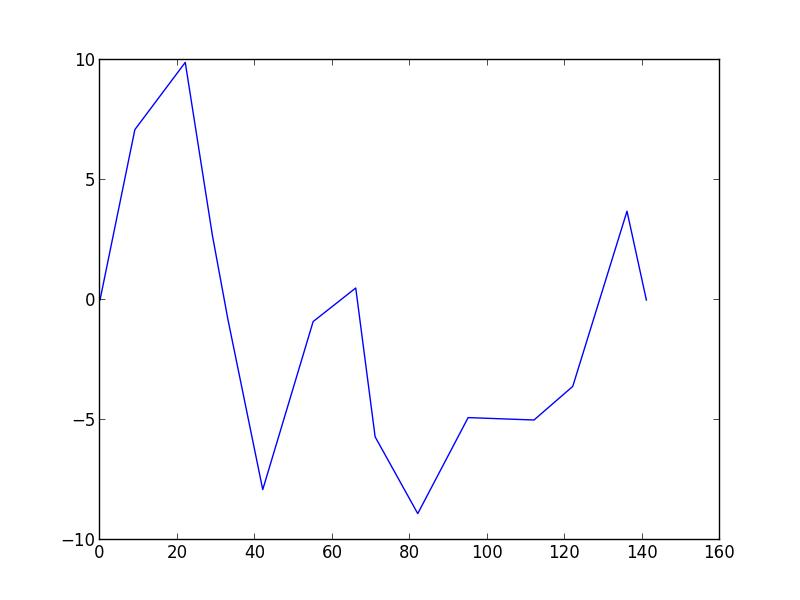
\includegraphics[width=.5\textwidth]{figure_1.png}
	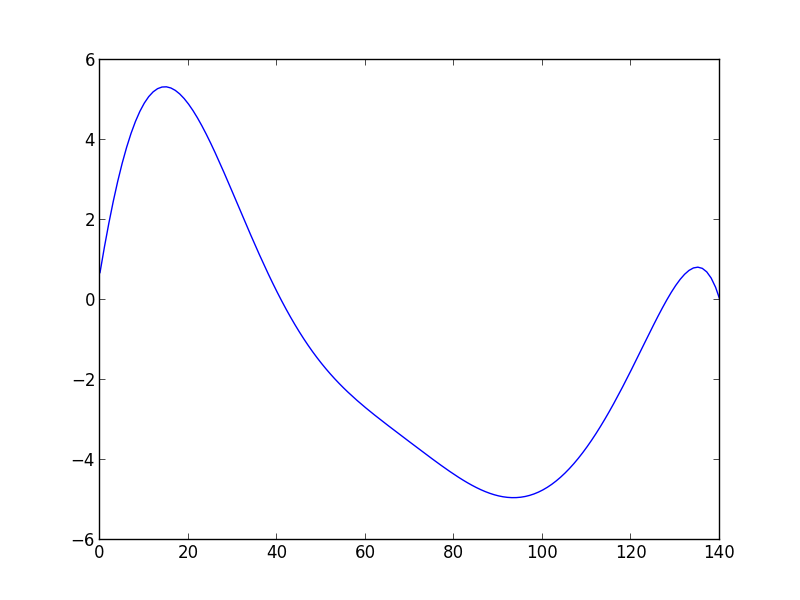
\includegraphics[width=.5\textwidth]{figure_2.png}
	\caption{Applying Bezier Smoothing to the discrete points}
\end{figure}

\subsection{Introduction of noise}
- Smoothing was too smooth\\
- Didn't look too natural \\
- Introduced a probability based addition or subtraction\\

\begin{figure}
	\centering
	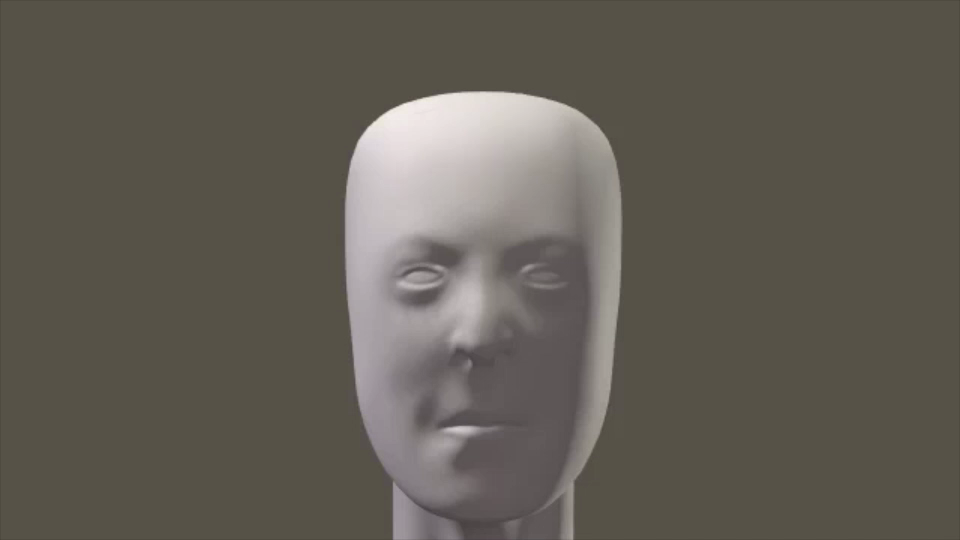
\includegraphics[width=.5\textwidth]{fightclub1.png}
%	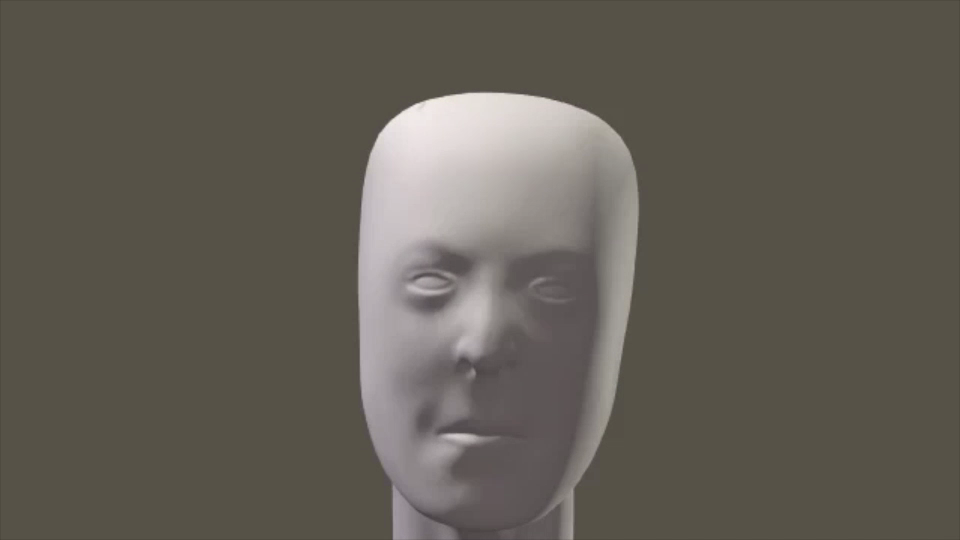
\includegraphics[width=.19\textwidth]{fightclub2.png}
	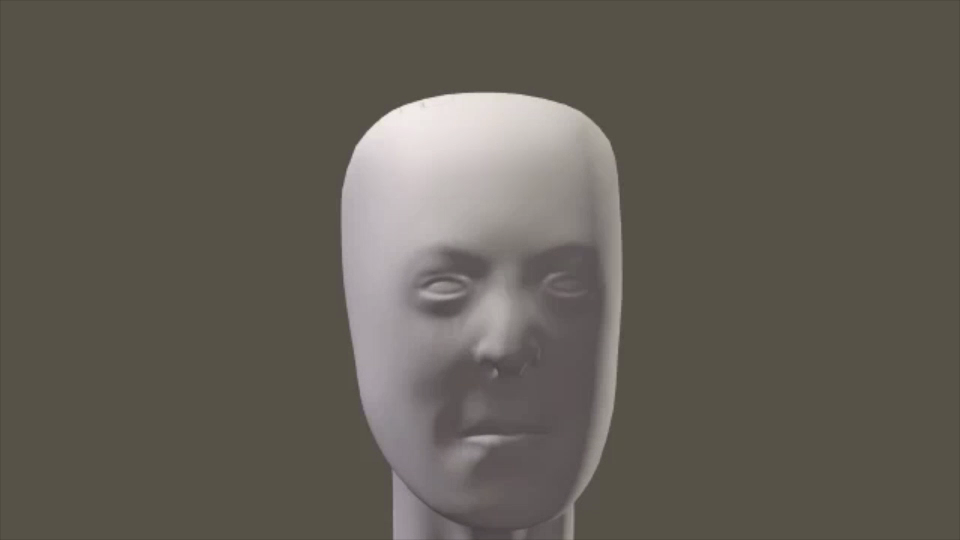
\includegraphics[width=.5\textwidth]{fightclub3.png}
	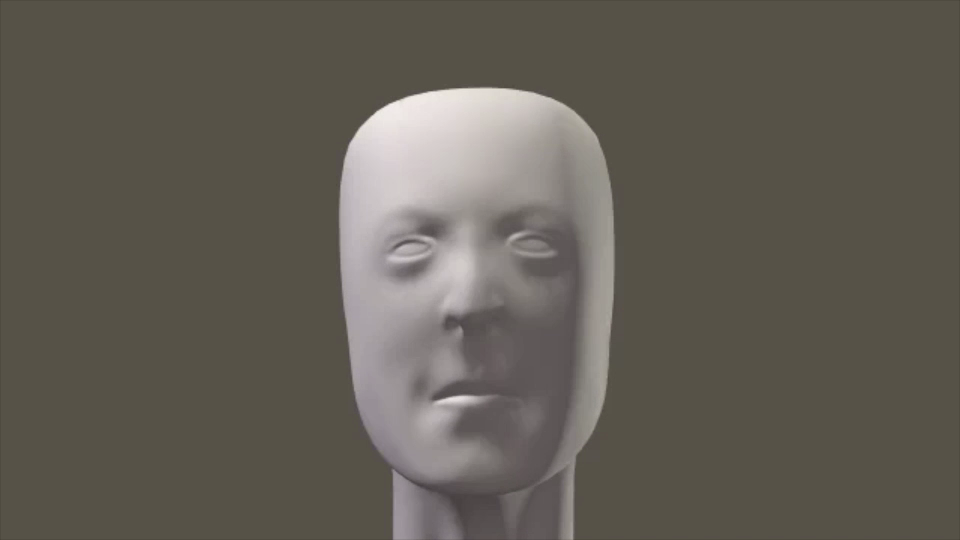
\includegraphics[width=.5\textwidth]{fightclub4.png}
%	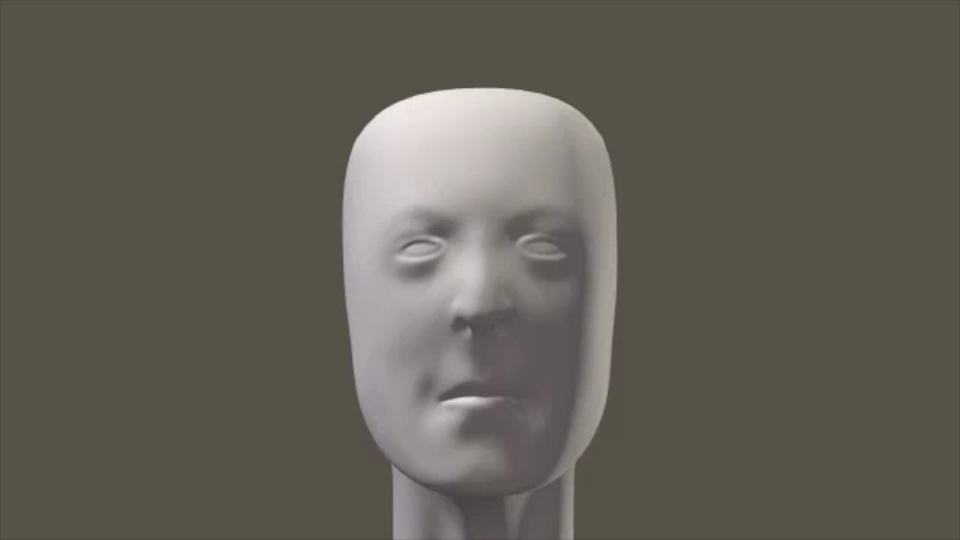
\includegraphics[width=.19\textwidth]{fightclub5.png}
	\caption{Output from random system}
\end{figure}

\section{Rule-Based System}

\subsection{Using the information form festival}

\subsection{Parametric Smoothing}
- Felt Bezier did not look like natural head motions \\
- Removed stop words as there is not a 1-1 mapping between words and head motions
- Comparison with data looked too smooth even with noise \\
- Moved towards First Order equations \\
- commonly used in electronics \\
- felt it aligned with recorded head motions more\\
	
% ============================================================= %
\chapter{Evaluation}

To evaluate the Text-Driven Head Motion System I performed both subjective analysis and objective analysis. The aim for the project was to develop a system which generates life-like talking heads with head motions that seem realistic and natural so it was important for humans to evaluate if the head motions were natural or not. Having a unit of measurement describing how close to the original head motions was also necessary in evaluating the system.

\section{Subjective Analysis}

\subsection{Outline}
- Volunteers\\
- 5 Video Clips of animated talking heads \\
- 3 from the TDTH system\\
- 2 taken from actual recordings \\
- All mapped to the same face \\
- Volunteers will be asked to rate on a scale of 1-100 how natural the head motions seem \\
- Focus only on the head motions \\
- Evaluating Only One Criteria
- Not told which are synthesised\\
- Not told about real recordings \\
- So volunteer does not know which were which\\

- Developed Web-based platform for subjective evaluation\\
- Using Python, Flask and HTML5\\
- Used Sliders going from 0-100 \\
- allowed higher precision \\


- Important to keep as much the same as possible\\
- Only change head motions\\
- Apply Dynamic Time Warping\\ 

\subsection{Preliminary Results and feedback}

- Performed evaluation with small number of volunteers \\

- Asked questions about the experience \\
- Difficulty of task \\
- Creepy / Uncanny Valley \\
- Adjust quality of videos \\
- Longer Videos \\ 

\subsection{Results}

- Taken on  board suggestions from preliminary \\
- 15 volunteers \\
- Good results for Random system \\
- Good results for rule-based system \\
- Bad results for ones taken from data \\

\subsection{Conclusions}


\section{Objective Analysis}

- Calculate difference in Euler angles\\
- Compare each system to two recordings due to lack of transcriptions\\

\subsection{Results}
% ============================================================= %
\chapter{Conclusions}

\section{System Overview}

\section{Discussion}

\subsection{Classification and Regression Trees}

\subsection{Data Driven System}

\section{Future Work}

\subsection{Expansion of techniques}

\subsection{Second Order Smoothing}
	
\bibliographystyle{plain}
\bibliography{diss}

\end{document}
